% Template for ICIP-2014 paper; to be used with:
%          spconf.sty  - ICASSP/ICIP LaTeX style file, and
%          IEEEbib.bst - IEEE bibliography style file.
% --------------------------------------------------------------------------
\documentclass{article}
\usepackage{spconf,amsmath,graphicx}

\usepackage{subfigure}

\usepackage{algorithmicx}
\usepackage[ruled]{algorithm}
\usepackage{algpseudocode}
\usepackage{array}
\usepackage{color}
\definecolor{purple}{rgb}{0.65,0,0.65}


% Example definitions.
% --------------------
\def\x{{\mathbf x}}
\def\L{{\cal L}}

% Title.
% ------
\title{Robust Interactive Image Segmentation via Iterative Refinement}
%
% Single address.
% ---------------
\name{$\text{Yao Peng}^1$, $\text{Juyong Zhang}^1$, $\text{Yancheng Yuan}^1$, $\text{Shuyuan Zhu}^2$ and $\text{Lu Fang}^1$}
\address{$^1$University of Science and Technology of China\\ $^2$University of Electronic Science and Technology of China}
%
% For example:
% ------------
%\address{School\\
%	Department\\
%	Address}
%
% Two addresses (uncomment and modify for two-address case).
% ----------------------------------------------------------
%\twoauthors
%  {A. Author-one, B. Author-two\sthanks{Thanks to XYZ agency for funding.}}
%	{School A-B\\
%	Department A-B\\
%	Address A-B}
%  {C. Author-three, D. Author-four\sthanks{The fourth author performed the work
%	while at ...}}
%	{School C-D\\
%	Department C-D\\
%	Address C-D}
%
\begin{document}
%\ninept
%
\maketitle
%
\begin{abstract}
Image segmentation with user inputs gets more and more popular in recent years and always performs better compared with automatic methods. However, existing interactive image segmentation methods still might fail if the image contains messy textures, or the user inputs are sparse or at inappropriate locations. In this paper, we propose a novel iterative refinement framework which leads to robust segmentation performance even with sparse and improper input strokes. Specifically, a geodesic distance based energy is introduced and combined with convex active contour model, and an iterative seeds refinement technique is put forward to handle the sparse input problem. Extensive experiments using real world images, and segmentation benchmark dataset show that our proposed method has superior performance compared with representative state-of-the-art methods.
\end{abstract}
%
\begin{keywords}
Interactive Image Segmentation, Seeds Refinement, Geodesic Distance, Convex Active Contour Model
\end{keywords}
%
\section{Introduction}
\label{sec:intro}
%
\subsection{Motivation}
%
In recent years, interactive image segmentation becomes more and more popular as it can produce more reliable segmentation result with the help of the information supplied by users. This type of interactive way is quite useful for many image editting problems and medical image processing applications. However, the performance of interactive image segmentation heavily depends on the quality and quantity of the inputs seeds supplied by the users.

In most of the existing methods, the regions without seeds might be assigned to incorrect labels. For an object with complex texture, the input seeds can not cover every sub-region of the interested object. These regions without seeds can not be segmented robustly. Moreover, the seeds are fixed during the whole segmentation process in most of existing methods. In other words, much information of former iterations are not involved in the following iterations and these regions without seeds can not be segmented robustly. In this paper, we try to propose a robust interactive image segmentation method to deal with these problems which are rarely considered before.
%
\subsection{Related Works}
%
In general, there are two categories of interactive image segmentation approaches: boundary-based and region-based ones. State-of-the-art region-based interactive segmentation algorithms include Graph Cut based methods \cite{boykov2001interactive, rother2004grabcut}, Random Walks(RW) based methods \cite{grady2006random, zhang2010diffusion}, and Geodesic methods \cite{bai2007geodesic, criminisi2008geos}. All these methods firstly convert an image into a weighted graph and then minimize an objective energy functional to produce the final segmentation. However, the Graph Cut algorithm is sensitive to the number of seeds, while the RW and Geodesic algorithms are sensitive to the locations of seeds \cite{sinop2007seeded}.
%

In 2007, Bresson et. al. \cite{bresson2007fast} proposed a convex active contour model based on the ``active contours without edges'' model~\cite{ChanV01} and ``Mumford-Shah'' model~\cite{Mumford89} to make use of both the boundary and the regional information. Recently, Nguyen et. al.\cite{nguyen2012robust} extended this model to interactive image segmentation, which is called constrained active contour model. They used the segmentation result of the Geodesic method \cite{bai2007geodesic} for contour initialization and foreground/background Gaussian Mixture Models(GMMs)\cite{rother2004grabcut} to represent the regional term.
%

The energy term in segmentation models is always composed by global energy term \cite{KassWT88,CasellesKS97} and local energy term \cite{levin2004colorization, lischinski2006interactive}. The former one relates each pixel to all samples and it can quickly propagate seeds through the image while the latter one involves more user interaction. Recently a new method proposed by Xu\cite{xu2013sparse} is based on iterative feature discrimination and it relates each pixel to part of the control samples. It successfully combine the effect of both global and local operators even with a small amount of user inputs.
\begin{figure}[htbp]
\begin{center}
%\fbox{\rule{0pt}{2in} \rule{.9\linewidth}{0pt}}
\subfigure[]{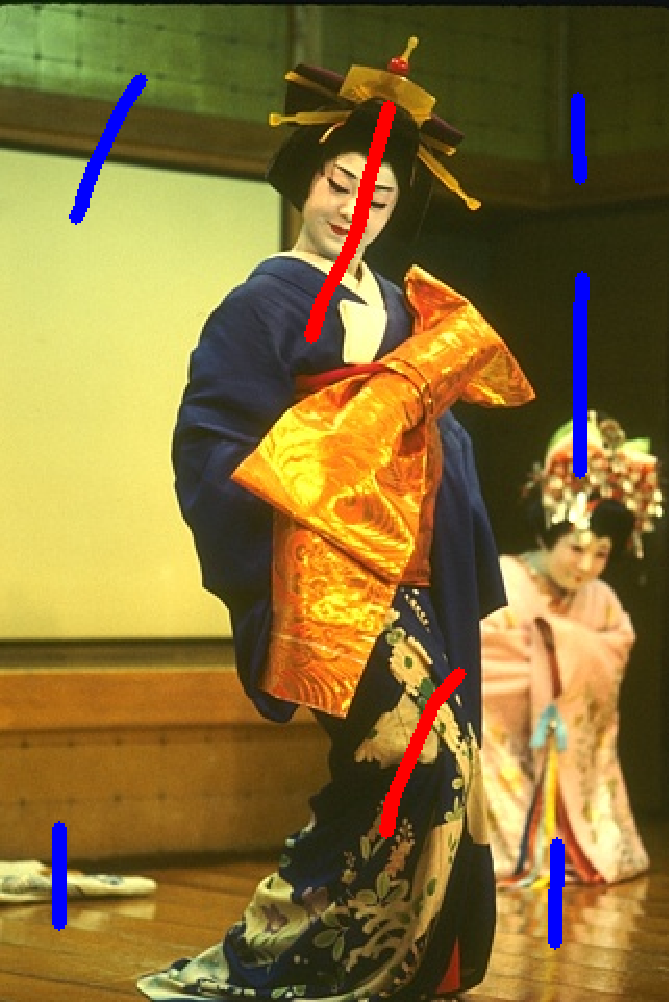
\includegraphics[width=0.23\linewidth]{Figures/1_a.pdf}}
\subfigure[]{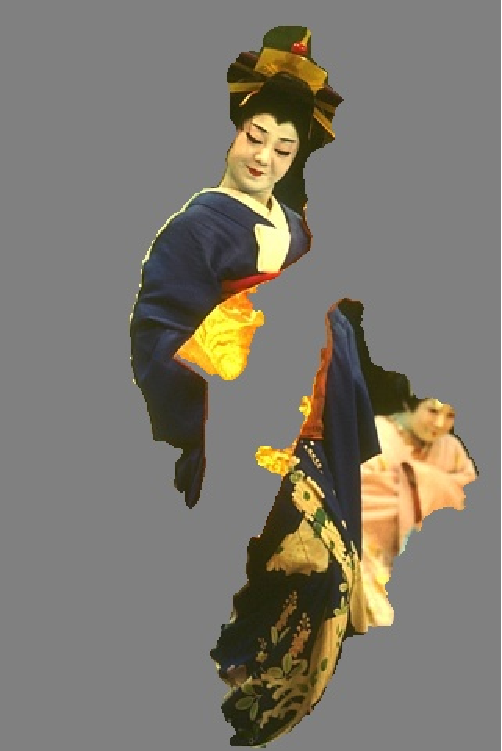
\includegraphics[width=0.23\linewidth]{Figures/1_b.pdf}}
\subfigure[]{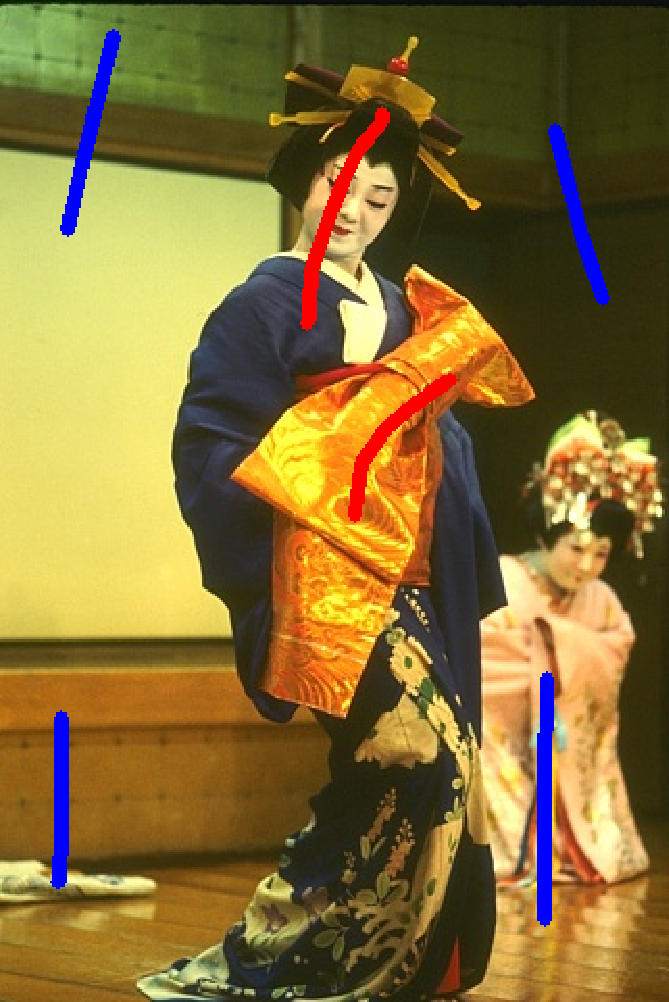
\includegraphics[width=0.23\linewidth]{Figures/1_c.pdf}}
\subfigure[]{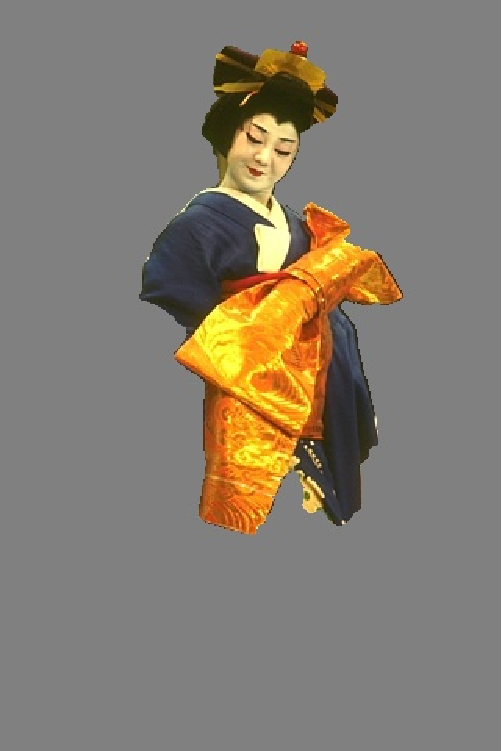
\includegraphics[width=0.23\linewidth]{Figures/1_d.pdf}}
\end{center}
\vspace{-2em}
   \caption{For images with complex color distribution, results of the model in \cite{nguyen2012robust} are quite different with different sparse input strokes. Here (b) is the segmentary result of input seeds in (a); (d) is the segmentary result of input seeds in (c).}
\label{fig:fig1}
\end{figure}
%

Through extensive experiments we find the crucial problems of existing methods are: 1) the results of segmentation are extremely sensitive to the locations and quantity of seeds; 2) these methods can barely work on images with complex color distribution or messy textures. Results of using a representative method \cite{nguyen2012robust} with different sparse user inputs are shown in Fig.~\ref{fig:fig1}. Obviously, the different performances in Fig.~\ref{fig:fig1}(b) and (d) indicate that the segmentation is sensitive to locations of seeds, especially without sufficient input strokes.
%
\subsection{Our Contributions}
%
Current interactive image segmentation methods mainly consider the color information like the tensity or their distributions, and the user supplied seeds are fixed and used only once. The fixed user inputs might result in uncertainties when the desired segmentation region does not contains input seeds. Besides, as mentioned in the motivation part, invariable seeds will lose some important information during the iterations in the segmentation procedure. In this paper, a new model with seeds refinement is proposed and performs much better, even for images with sparse inputs.
%
In summary, the main contributions of this paper are:
\begin{itemize}
\item A geodesic energy term is introduced and combined with convex active contour model to enhance the weightiness of those seed regions.
\item A seeds refinement technique is proposed to enhance the reliable segmentation results, and use them to guild the unreliable part segmentation.
\end{itemize}
Experiments on MSRC dataset show that the proposed method produces high quality segmentation results even with few user inputs.
%

The rest of the paper is organised as follows: In Section~\ref{sec:geoenergy} we explain the new Geodesic energy term together with the constrained active contour model as well as the proposed iterative seeds refinement scheme. In Section~\ref{sec:Exp}, we verify our method by showing some representative results and discussions. The conclusions are given in Section~\ref{sec:Conc}.
%
\vspace{-3mm}
\section{Robust Interactive Image Segmentation}
\label{sec:geoenergy}
In this section, we will first introduce how to modify the Constrained Active Contour Model to incorporate the seeds location information. Then the interative seeds refinement strategy is proposed to handle the low quality and small quantity of input seeds problem.
%
\subsection{Modified Constrained Active Contour Model}
%
Active contour model~\cite{GoldsteinBO10,nguyen2012robust} gets big success in image segmentation. However the seed locations are not emphasized in existing models, and thus the regions without seeds might be assigned with incorrect labels. To handle this problem, a geodesic energy term is added to enhance the weightiness of those seed regions. The proposed model is formulated as
\begin{equation} \label{eq:newmodel}
\begin{array}{rl}
   \underset{u\in[0,1]}{ \min}  & \int_\Omega{g_b|\nabla u|+\lambda_1h_ru+\lambda_2(d_F-d_B)u^2dx} \\
   \textrm{s.t} & u(x) = 1 ~~~~~~ \textrm{if $x\in F$}\\
& u(x) = 0  ~~~~~~ \textrm{if $x\in B$},
\end{array}
\end{equation}
%Here we introduce the called geodesic term $(d_F-d_B)u^2$ as part of the modified constrained active contour model to enhance the performance, where $d_F$ and $d_B$ is the geodesic distance function for a pixel to foreground and background \cite{bai2007geodesic}; $u$ is a foreground weight function in the image domain $\Omega$, which decides the segmentation result; $\lambda_1$ and $\lambda_2$ are used to balance the proportion of each part. Specifically, let $Pr(c_x|F)$, $Pr(c_x|B)$ denote the probabilities of the GMMs. The likelihood of a pixel $x$ with color $c_x$ belonging to the foreground becomes $P_F(c_x)={Pr(c_x|F)}/{(Pr(c_x|F)+Pr(c_x|B))}$, where $F$(or $B$) is the set of pixels in foreground(or background). $P(x)=D_B(x)/(D_F(x)+D_B(x))$ is assigned to $u(x)$ as initialization. $g_b$ and $h_r$ are the same as in \cite{nguyen2012robust}, which describe the boundary and regional properties of the image. They are defined in Eq.~\ref{eq:gb} and Eq.~\ref{eq:hr}.
%\begin{equation} \label{eq:gb}
%    g_b=\beta\cdot g_c+(1-\beta)\cdot g_e
%\end{equation}
%\begin{equation} \label{eq:hr}
%    h_r(x)=\alpha(P_B(c_x)-P_F(c_x))+(1-\alpha)(1-2P(x))
%\end{equation}
%where $g_c$ and $g_e$ are edge detection results of $P_F(c_x)$ and the original image, respectively.
%
where $\lambda_1$ and $\lambda_2$ are two trade-off parameters. $u$ is a probability function defined on image domain $\Omega$, which has a value between 0 and 1 at each pixel location $x$ in the image. Set $F$(or $B$) is the pixels in foreground(or background). The segmented region is obtained by thresholding the function $u$. Different from the models in \cite{GoldsteinBO10,nguyen2012robust}, the geodesic energy term $(d_F-d_B)u^2$ is added to the modified constrained active contour model to enhance the performance, where $d_F(x)$ and $d_B(x)$ are the geodesic distance of pixel $x$ to foreground and background \cite{bai2007geodesic} separately.

$g_b$ and $h_r$ in our model are the same as in \cite{nguyen2012robust}, which describe the boundary and regional properties of the image. They are defined as:
\begin{equation} \label{eq:gb}
    g_b = \beta\cdot g_c + (1 - \beta)\cdot g_e
\end{equation}
\begin{equation} \label{eq:hr}
    h_r(x) = \alpha(P_B(c_x) - P_F(c_x)) + (1 - \alpha)(1 - 2P(x))
\end{equation}
where $g_c$ and $g_e$ are edge detection results of $P_F(c_x)$ and the original image, respectively. $Pr(c_x|F)$, $Pr(c_x|B)$ denote the probabilities of the Gaussian Mixture Models(GMMs). The likelihood of a pixel $x$ with color $c_x$ belonging to the foreground becomes $P_F(c_x)={Pr(c_x|F)}/(Pr(c_x|F)+Pr(c_x|B))$. $P(x)=D_B(x)/(D_F(x)+D_B(x))$ is assigned to $u(x)$ as initialization.

\begin{figure}[htbp]
\centering
\subfigure{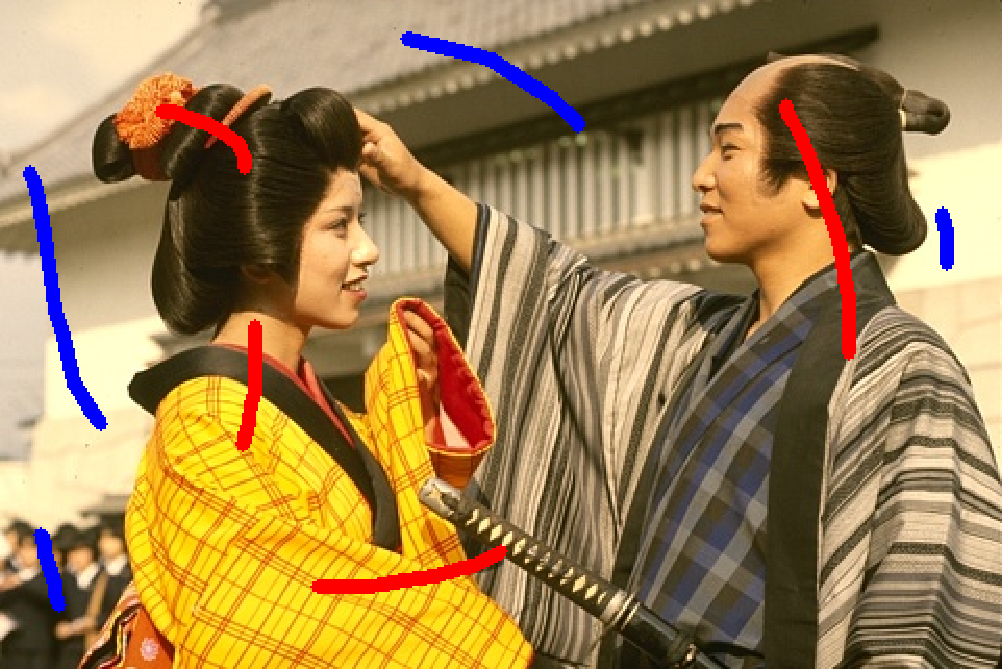
\includegraphics[width=4cm]{Figures/2_a.pdf}}
\subfigure{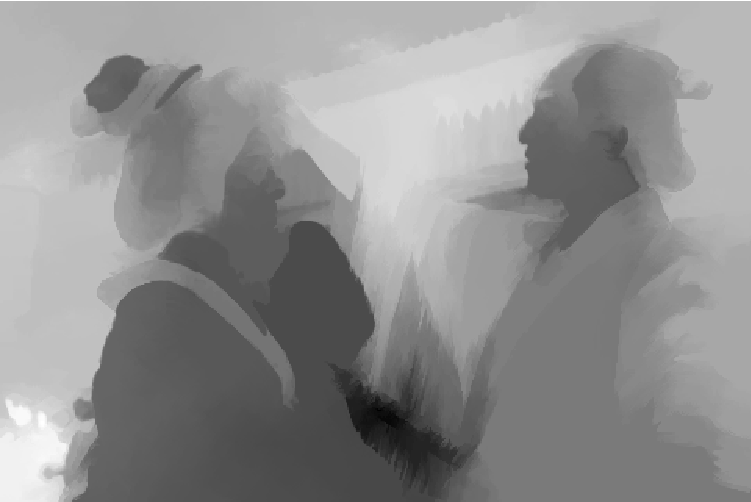
\includegraphics[width=4cm]{Figures/2_b.pdf}}
   \caption{ (Left) A sample image with sparse inputs; (Right) the visualization of $d_F-d_B$.}
\label{fig:fig2}
\end{figure}

The newly added geodesic energy term in model~\eqref{eq:newmodel} increases the weight of the region near the seeds. If $d_F(x) < d_B(x)$, it means that pixel $x$ is closer to the foreground seeds from the perspective of geodesic distance, and thus $u(x)$ is supposed to assign a larger value. This term magnify the effect of the seed regions. As shown in Fig.~\ref{fig:fig2}, the visualization of $d_F-d_B$ is showed. The week edges such as the texture does not increase the geodesic distance. Thus the region without seeds but near with the seeds region in the geodesic distance can obtain a more proper segmentation result.

\subsubsection{Numerical algorithm}
To solve Eq.~\eqref{eq:newmodel}, we first introduce an auxiliary variable $d$ to substitute $\nabla u$ and rewrite ~\eqref{eq:newmodel} as
\begin{equation}\label{eq:rewrite of newmodel}
\begin{array}{rl}
   \underset{u\in[0,1]}{ \min}  & \int_\Omega{g_b|d|+\lambda_1h_ru+\lambda_2(d_F-d_B)u^2dx} \\
   \textrm{s.t} & d = \nabla u\\
& u(x) = 1 ~~~~~~ \textrm{if $x\in F$}\\
& u(x) = 0  ~~~~~~ \textrm{if $x\in B$},
\end{array}
\end{equation}
Then we can optimize the problem via Split Bregman~\cite{GoldsteinO09} as following:
\begin{equation} \label{eq:bregmanmodel}
\begin{aligned}
    (u^{k+1},d^{k+1})=arg \min_{u\in[0,1],d}\int_\Omega g_b|d|+\lambda_1h_ru+ \\
    \lambda_2(d_F-d_B)u^2+\frac{\mu}{2}|d^k-\nabla u-b^k|^2dx
\end{aligned}
\end{equation}
%
\begin{equation}
    b^{k+1}=b^k+\nabla u^{k+1}-d_{k+1}
\end{equation}
where superscript $k$ indicates the iteration index and $b$ is the dual variable. Based on the Euler-Lagrange differential equation, the value of $u$ can be solved by a Gauss-Seidel iterate method as
\begin{equation} \label{eq:GS}
    \mu\nabla u-2\lambda_2(d_F-d_B)u=\lambda_1h_r+\mu \mathbf{\mathrm{div}}(d^k-b^k),
\end{equation}
where $\mathbf{\mathrm{div}}$ is the divergence operator.
%
The minimum solution of $d$ value in Eq.~\eqref{eq:bregmanmodel} can be obtained by soft-thresholding
\begin{equation}
    d^{k+1}=\frac{\nabla u^{k+1}+b^k}{|\nabla u^{k+1}+b^k|}\max(|\nabla u^{k+1}+b^k|-\mu^{-1}g_b, 0)
\end{equation}
%
%
\subsection{Iterative Seeds Refinement}
%
In existing interactive image segmentation methods, the final segmentation result is decided by optimizing the proposed energy once with the initial user inputs. However, when the user input strokes are sparse or its locations are inappropriate, the complex objects are hardly to be segmented correctly. We propose to apply model~\eqref{eq:newmodel} to calculate the $u(x)$ multiple times by iteratively refining the seeds. With the newly updated seeds based on the optimized $u(x)$ value, we update the foreground/backgroud GMMs and recalculate the geodesic distance for every pixel to the updated seeds in each iteration. And then, the probability function $u(x)$ is recomputed by Eq.~\eqref{eq:newmodel}. This iteration is continued until the proportion of seed regions exceeds the predefined threshold. The final segmentaiton can be got through applying the threshold $T$ on the final $u(x)$. The seeds refinement and model's updating process are illustrated in Fig.~\ref{fig:pipeline} and our demo \cite{demo}.
\begin{figure}[t]
\begin{center}
%\fbox{\rule{0pt}{2in} \rule{.9\linewidth}{0pt}}
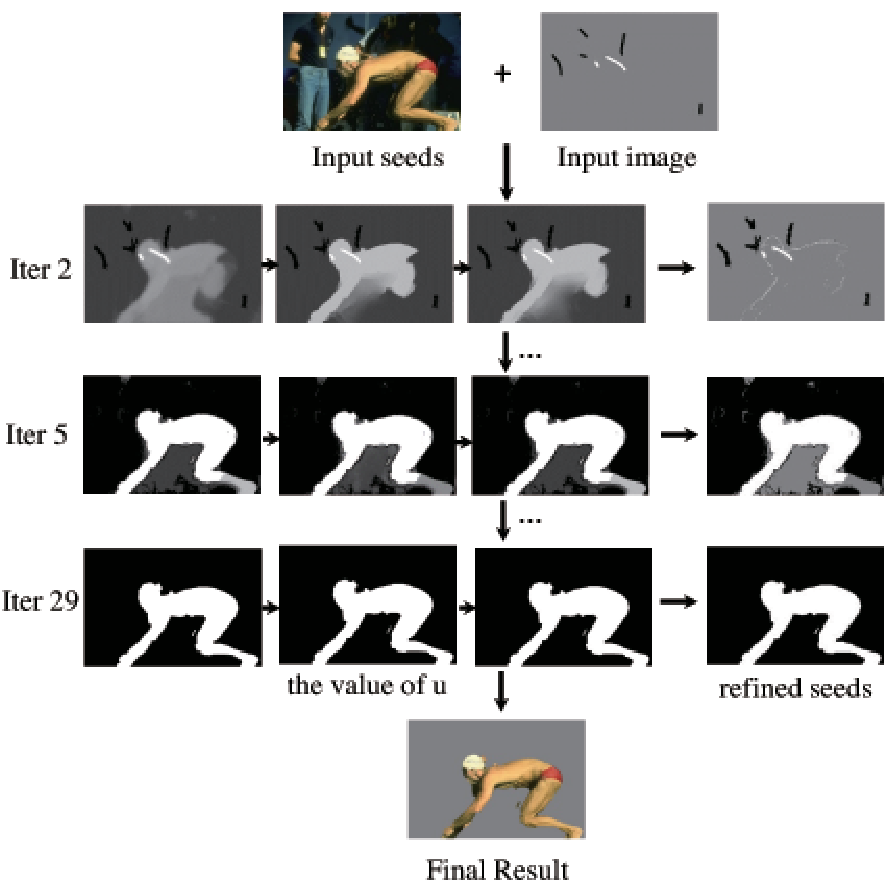
\includegraphics[width=0.8\linewidth]{Figures/pipe.pdf}
\end{center}
\vspace{-2em}
   \caption{Pipeline of our proposed method. The white pixels represent foreground seeds and the black represent background. In each iteration, the $u$ value is gradully refined as shown in each row, and the seeds are updated based on the optmized $u$ value.}
\label{fig:pipeline}
\end{figure}

Instead of segmenting images based on the initial input seeds in the model whose energy function is minimized only once, we make full use of the information which can generate the new seed regions properly and then the active contour model is updated. The more seeds input to the model, the more regions can be determined with high assurance. We iteratively update the segmentation results by solving the model multiple times with refined seeds. Fig~\ref{fig:figgeoiter} indicates obviously that with more iterations, the better visual results are achieved.
%\begin{algorithm}[htbp]
   % \caption{Seed regions growing and Model Updating.}
%    \begin{algorithmic}[1]
%        \State set $sr=\frac{\#\{seed regions\}}{\#\{image demain\}}$. $th_{sr}$ is stopping criterion of iteration.
%        \While ~~$sr<th_{sr}$
%            \State Calculate GMMs from seeds, $P_F(x)$, $P_B(x)$
%            \State Calculate $D_F(x)$ and $D_B(x)$, then update $P(x)$
%            \State Update $g_b$ and $h_r$
%            \State Obtain optimal $u(x)$ by Split Bregman method
%            \State Update $\{Foreground Seeds|u(x)>ut_F\}$ and $\{Background Seeds|u(x)>ut_B\}$, where $ut_F$ and $ut_B$ decide the boundary of seed regions growing.
%        \EndWhile
%        \State $\{Foreground|u(x)>T\}$
%    \end{algorithmic}
%    \label{algorithm:alggeoiter}
%\end{algorithm}
%
\begin{figure}[htbp]
    \centering
        \subfigure[seeds image]{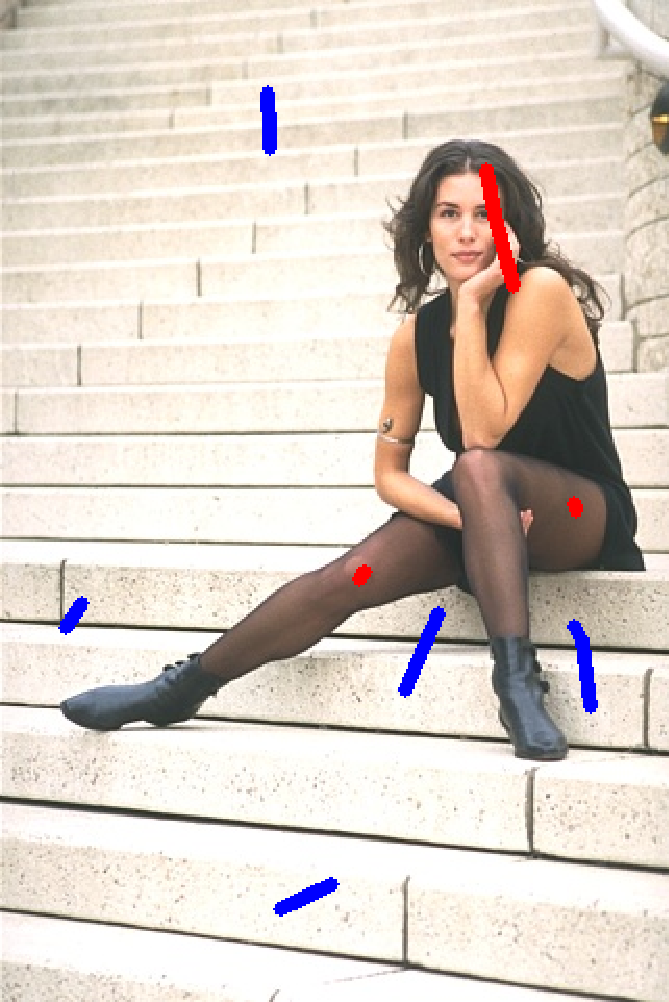
\includegraphics[width=2cm]{Figures/3a_1.pdf}}
        \subfigure[iter=1]{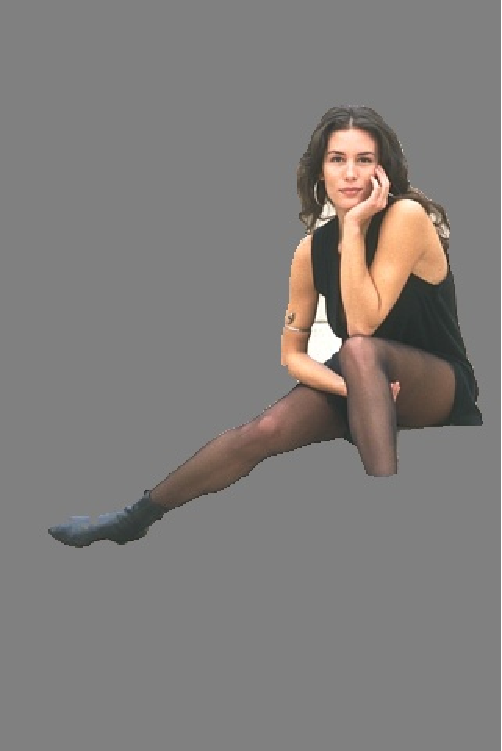
\includegraphics[width=2cm]{Figures/3a_2.pdf}}
        \subfigure[iter=5]{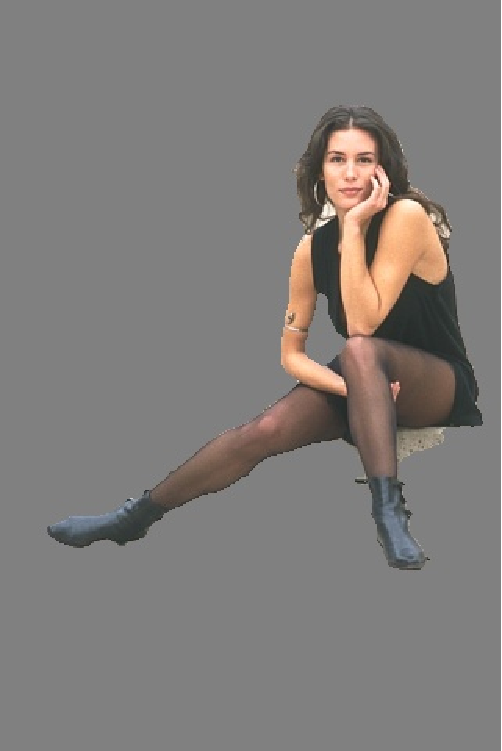
\includegraphics[width=2cm]{Figures/3a_3.pdf}}
        \subfigure[iter=27]{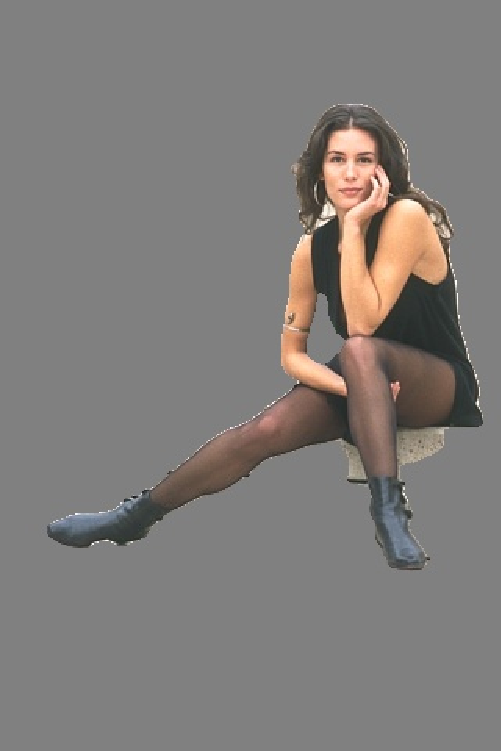
\includegraphics[width=2cm]{Figures/3a_4.pdf}}
   \caption{The results at different times of iterations for the image with complex color distribution and texture.}
\label{fig:figgeoiter}
\end{figure}
%

\vspace{-5mm}
\section{Experimental Results and Discussions}
\label{sec:Exp}
\vspace{-2mm}

In the experiments, the $\lambda_{1}$ is set to 100, which is same with the setting in~\cite{nguyen2012robust}. We also evaluate different $\lambda_{2}$ values. When the $\lambda_2$ is too small, the geodesic energy does not take important effect, while large value makes the seed locations dominant too much. For all the expterimental results, we set $\lambda_2$ to 1000.

%\begin{figure}[htbp]
%\centering
%\subfigure[$\lambda_2=0$]{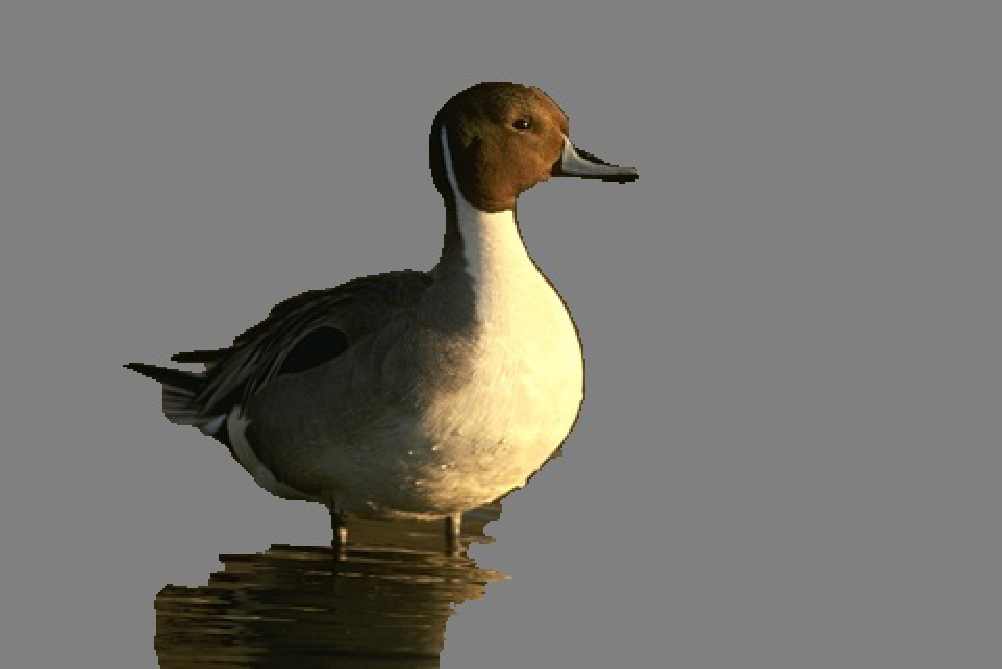
\includegraphics[width=0.23\linewidth]{Figures/6_a.pdf}}
%\subfigure[$\lambda_2=500$]{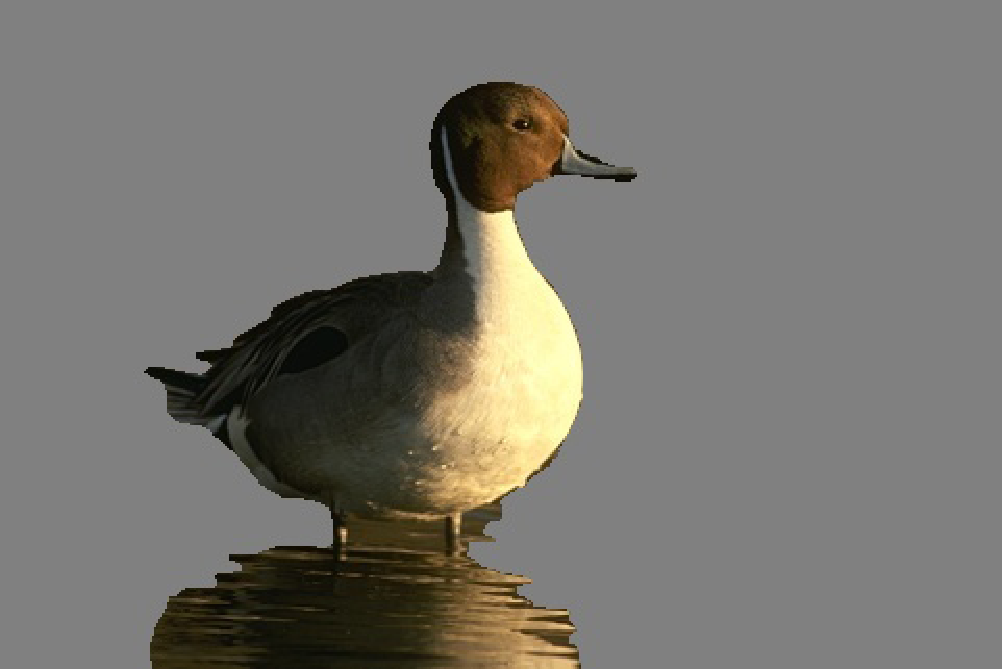
\includegraphics[width=0.23\linewidth]{Figures/6_b.pdf}}
%\subfigure[$\lambda_2=1000$]{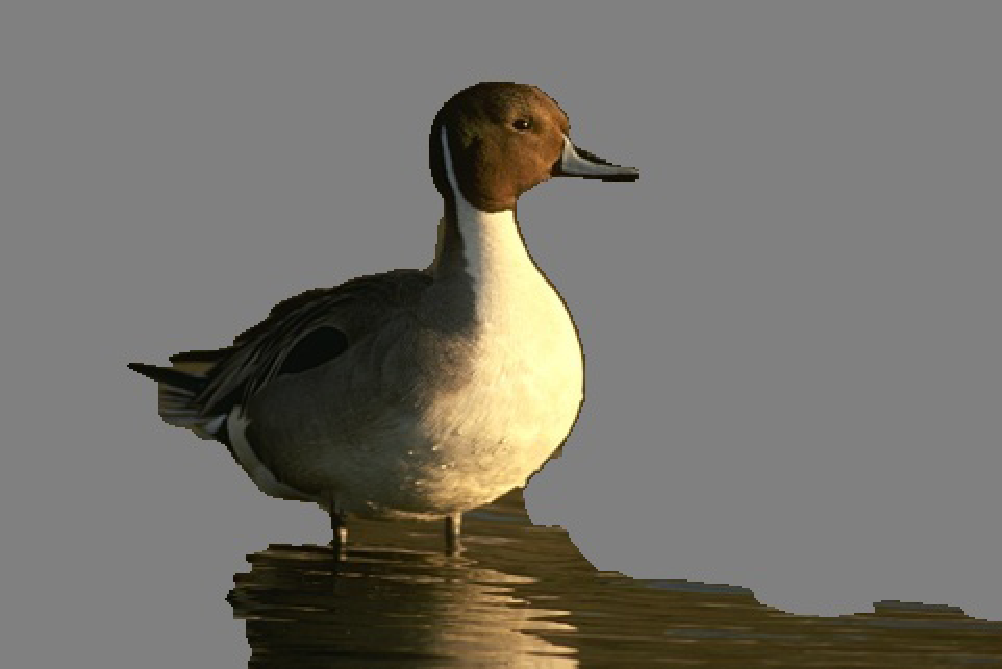
\includegraphics[width=0.23\linewidth]{Figures/6_c.pdf}}
%\subfigure[$\lambda_2=5000$]{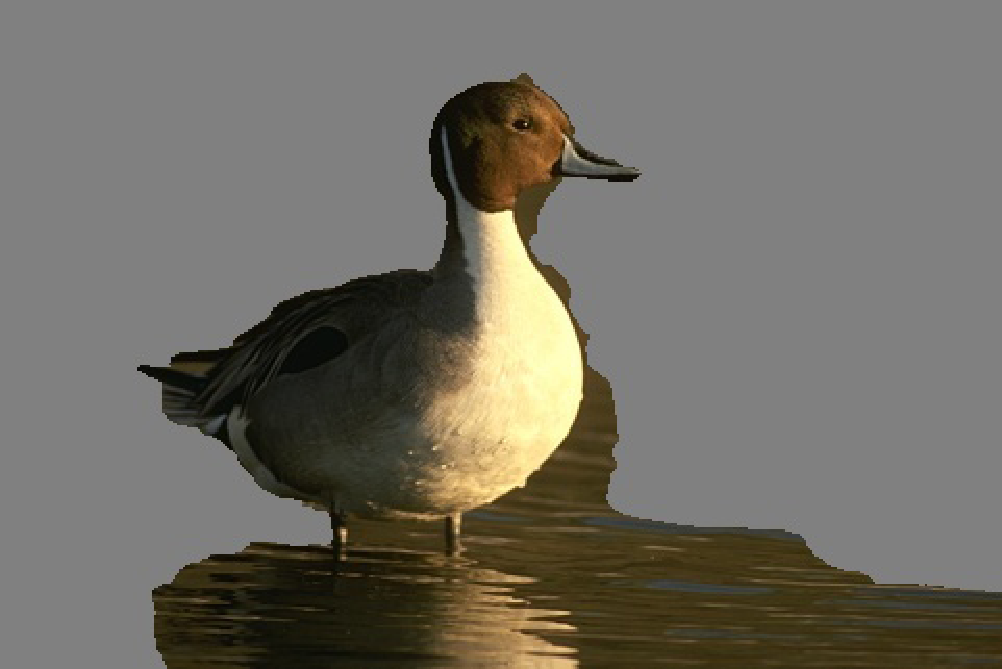
\includegraphics[width=0.23\linewidth]{Figures/6_d.pdf}}
%\vspace{-1em}
%   \caption{The comparison among different values of $\lambda_2$}
%\label{fig:fig6}
%\end{figure}
%
Fig.~\ref{fig:fig4} describes the segmentation results with sparse inputs on image with complex foreground and background. Here the sparse inputs mean that we only choose at most 1\% pixels of the whole image. According to Fig.~\ref{fig:fig4}, we can find that the results with our proposed model get better and better with more iterations, and results generated by the model in \cite{nguyen2012robust} are not good because of the complex images and the low quality and small quantity of the input seeds.

With the geodesic energy term, the texture structure around with foreground seeds can benefit the regions which are in the local area of seeds. In the cases of similar foreground and background, the method in \cite{nguyen2012robust} hardly finds the exact cutting contour, and even entirely fail in some particular cases with only segmenting the stroke regions, like the third example in Fig.~\ref{fig:fig4}. While with more iterations in our proposed method, the segmentation gets better and better as shown in the last column of Fig.~\ref{fig:fig4}.
\begin{figure}[!htb]
\begin{center}
\vspace{-1mm}
\subfigure{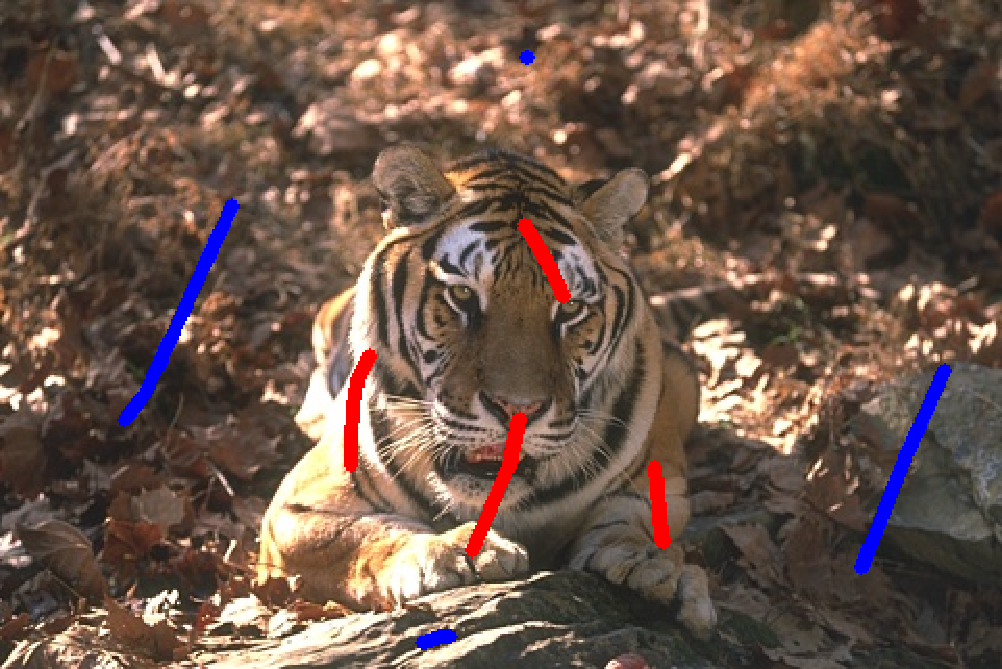
\includegraphics[width=0.22\linewidth]{Figures/4a_0.pdf}
            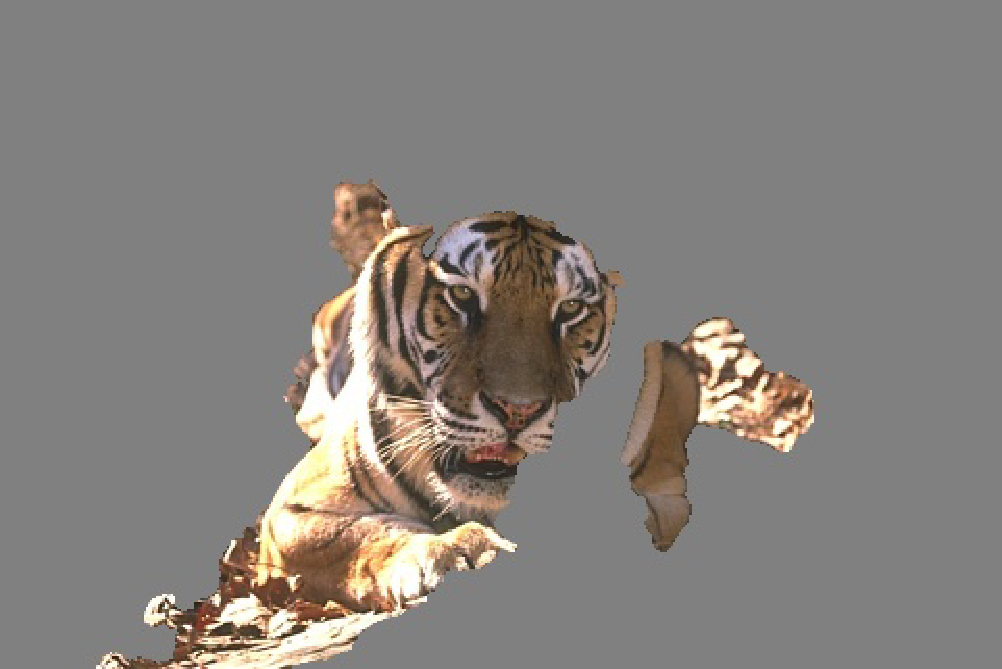
\includegraphics[width=0.22\linewidth]{Figures/4a_1.pdf}
            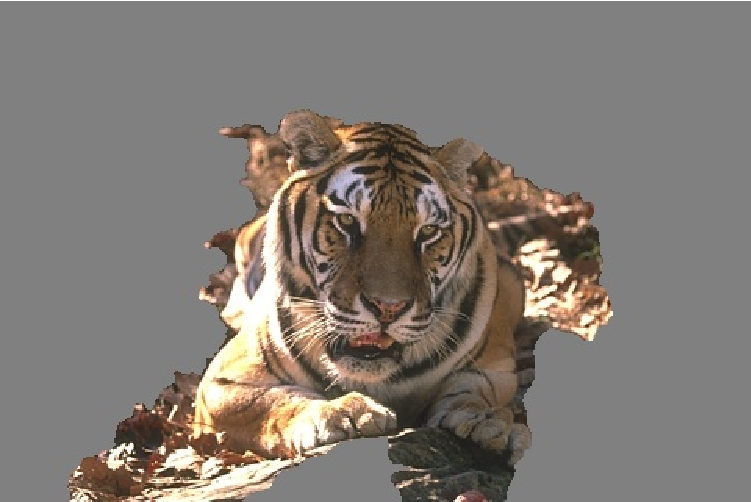
\includegraphics[width=0.22\linewidth]{Figures/4a_2.pdf}
            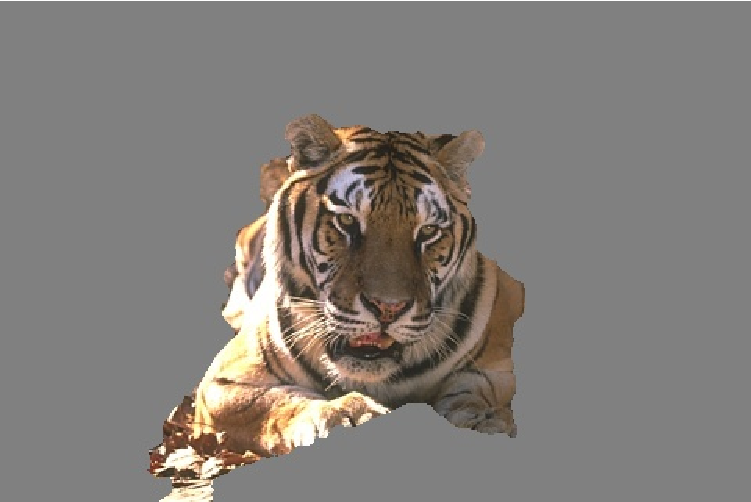
\includegraphics[width=0.22\linewidth]{Figures/4a_3.pdf}}
            \subfigure{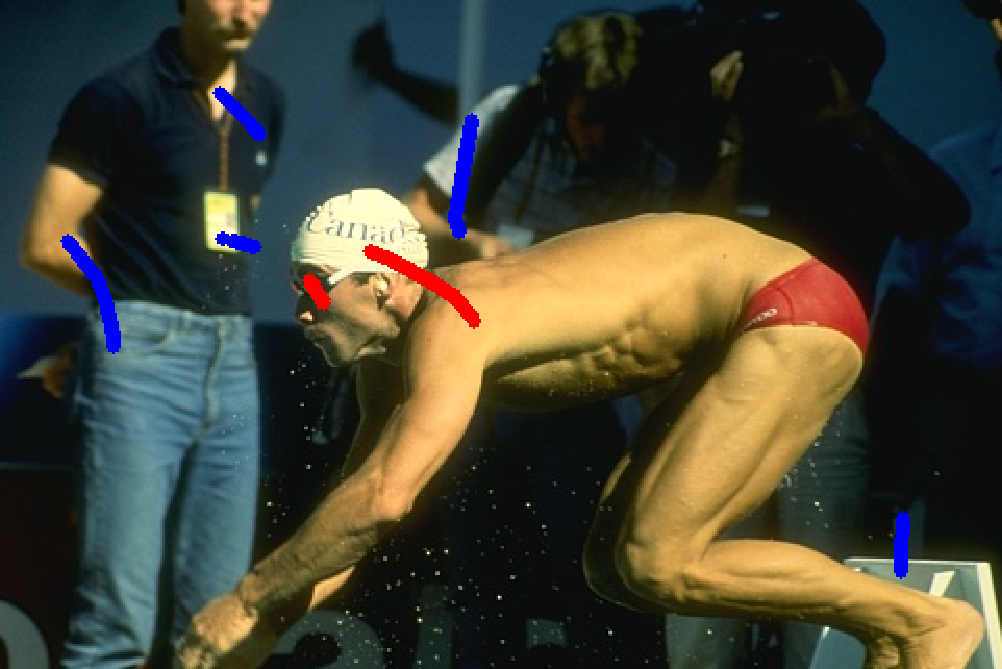
\includegraphics[width=0.22\linewidth]{Figures/4b_0.pdf}
            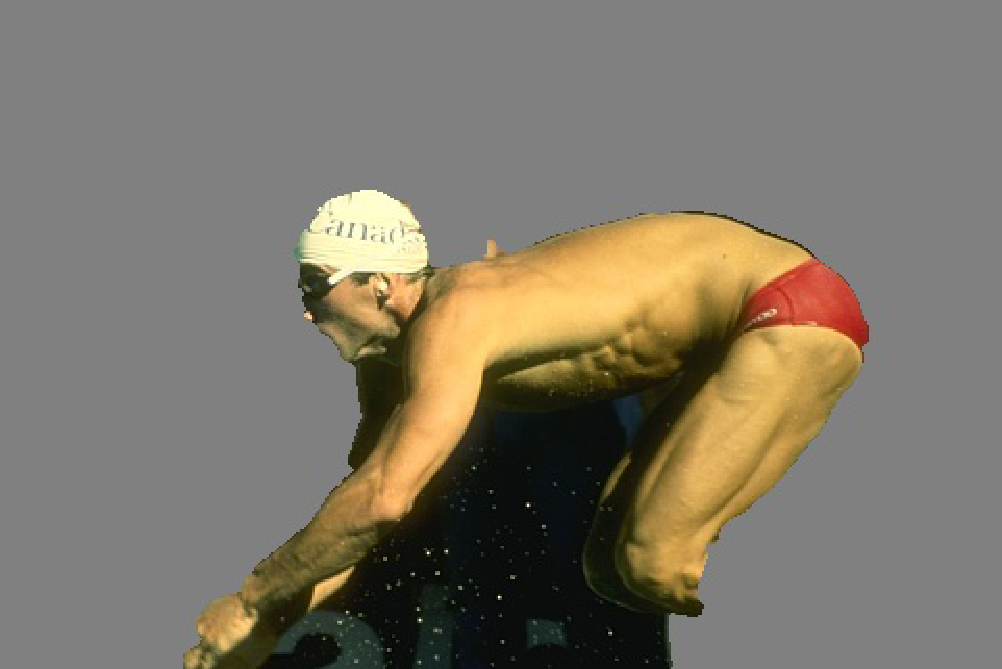
\includegraphics[width=0.22\linewidth]{Figures/4b_1.pdf}
            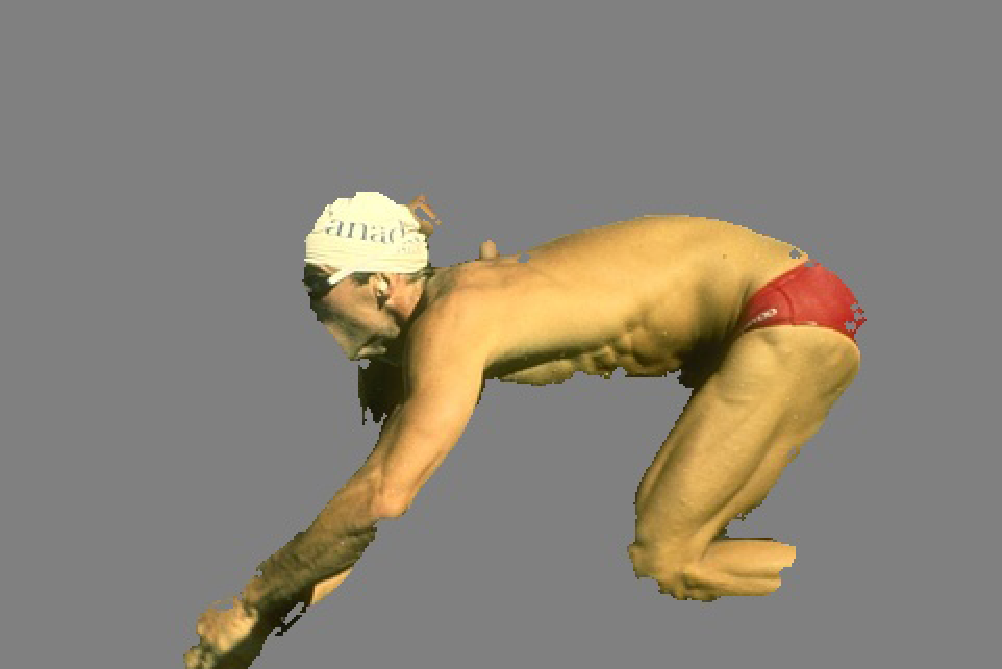
\includegraphics[width=0.22\linewidth]{Figures/4b_2.pdf}
            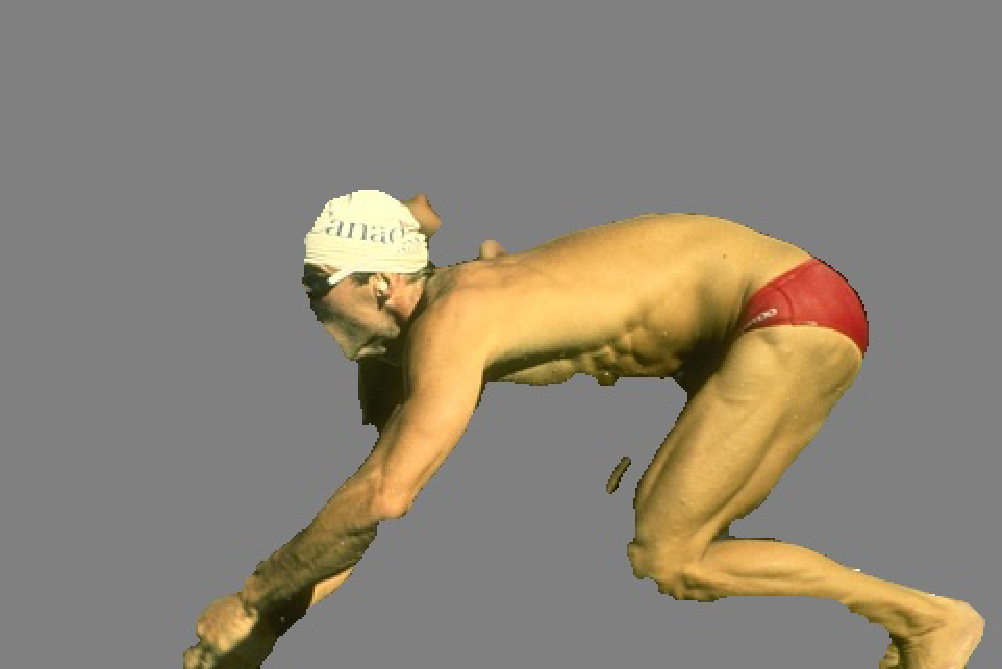
\includegraphics[width=0.22\linewidth]{Figures/4b_3.pdf}}
            \subfigure{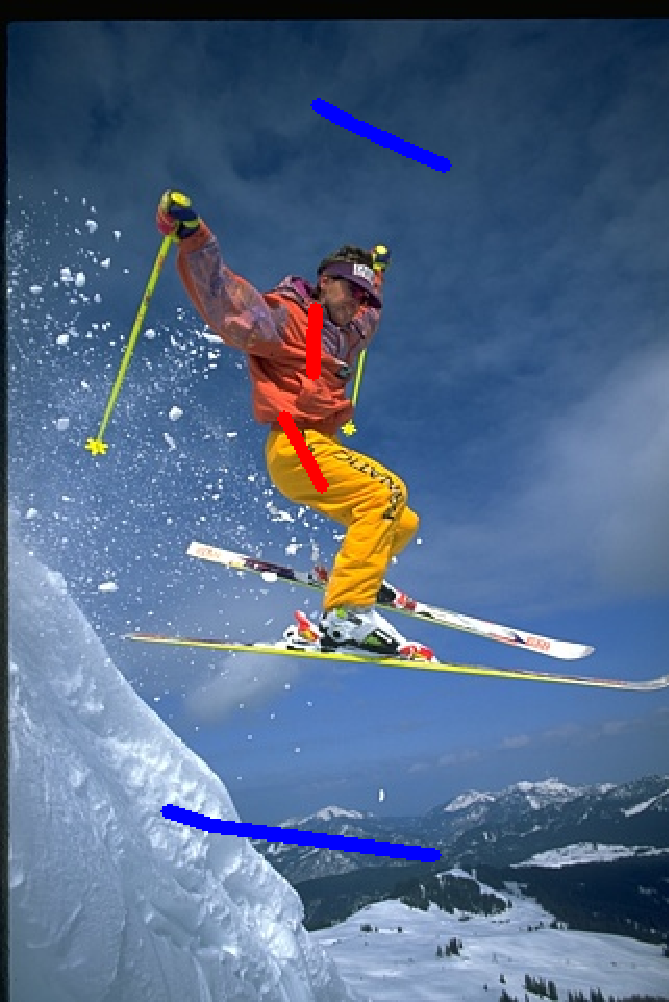
\includegraphics[width=0.22\linewidth]{Figures/4c_0.pdf}
            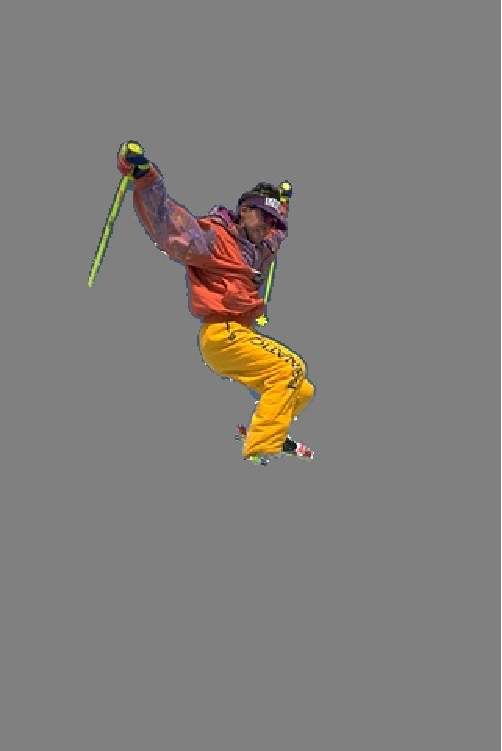
\includegraphics[width=0.22\linewidth]{Figures/4c_1.pdf}
            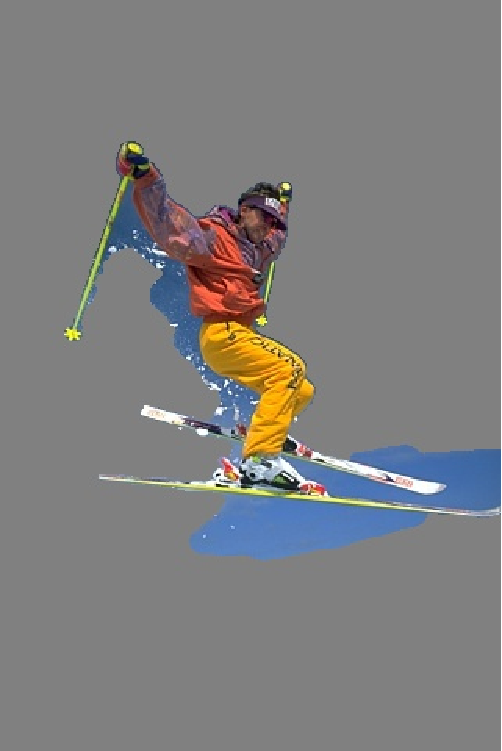
\includegraphics[width=0.22\linewidth]{Figures/4c_2.pdf}
            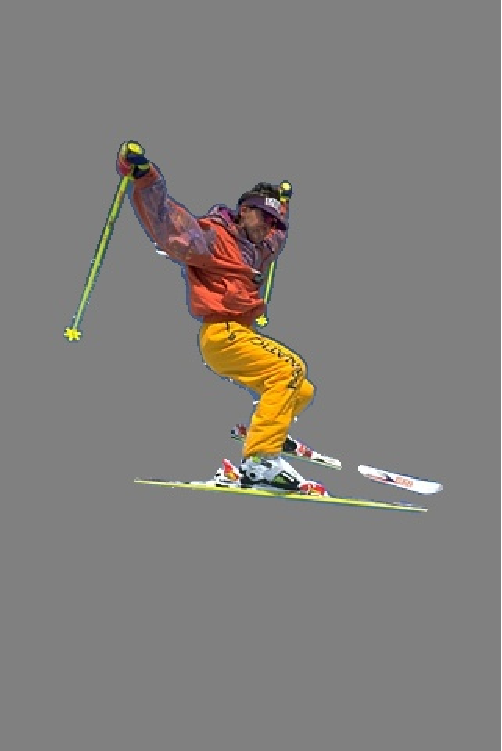
\includegraphics[width=0.22\linewidth]{Figures/4c_3.pdf}}
            \subfigure{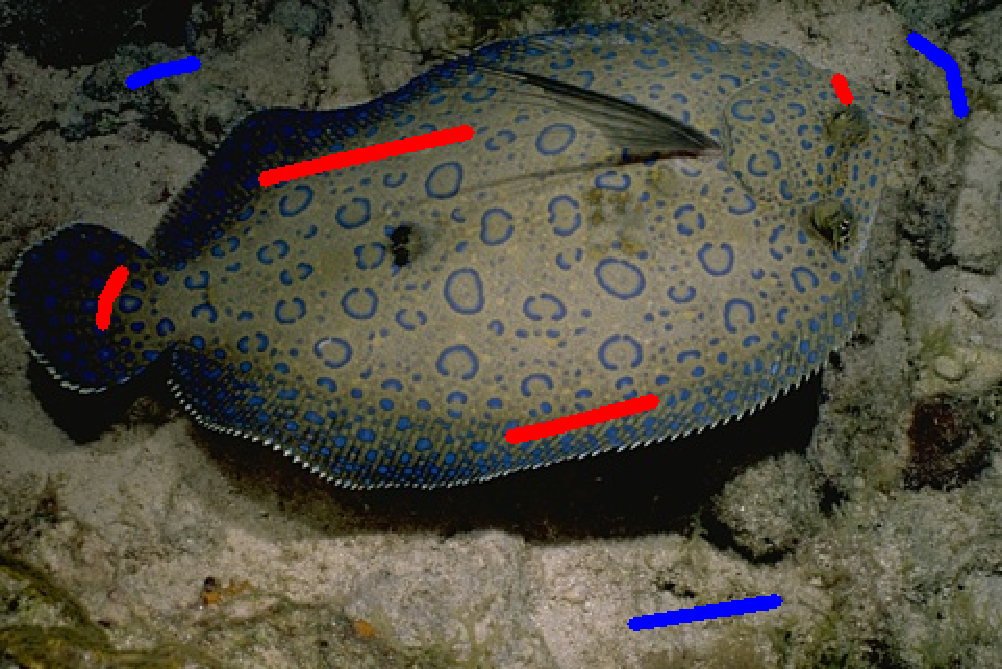
\includegraphics[width=0.22\linewidth]{Figures/4d_0.pdf}
            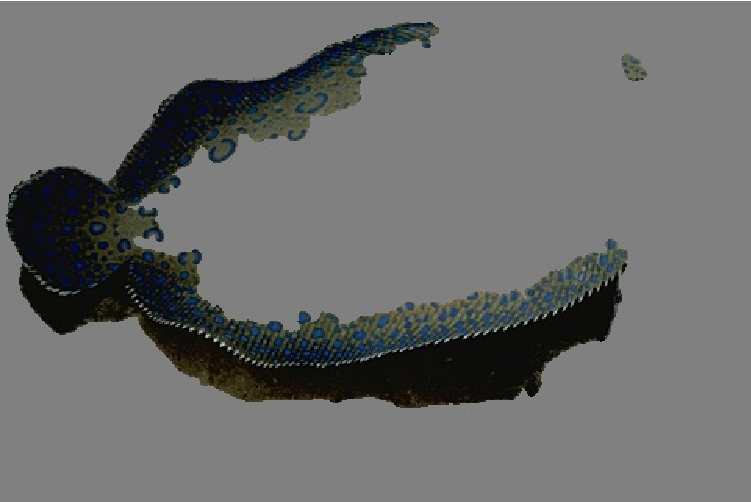
\includegraphics[width=0.22\linewidth]{Figures/4d_1.pdf}
            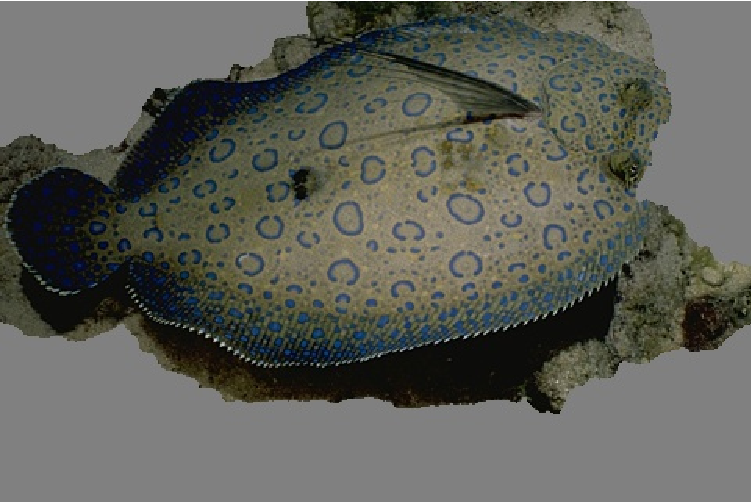
\includegraphics[width=0.22\linewidth]{Figures/4d_2.pdf}
            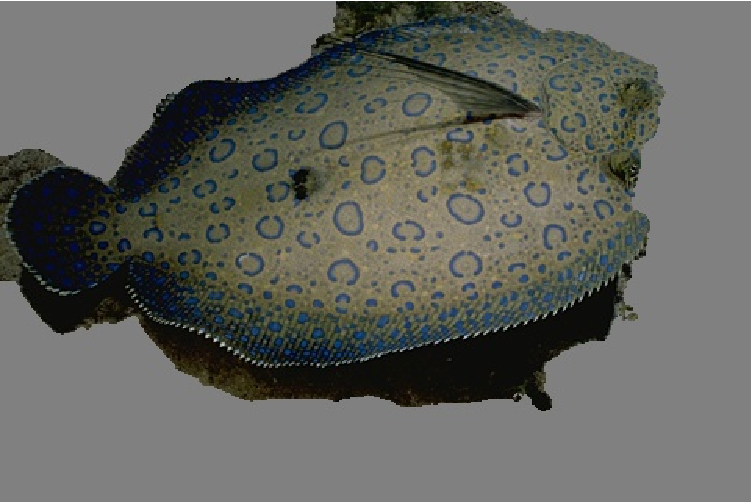
\includegraphics[width=0.22\linewidth]{Figures/4d_3.pdf}}
\vspace{-5mm}
\end{center}
   \caption{Segmentation results on complex images with sparse strokes. The second column are the results of \cite{nguyen2012robust}. The third column shows the results of model~\eqref{eq:newmodel}. The last column shows the final results until the seed refinement stops.}
\label{fig:fig4}
\end{figure}

In addition, our model is robust to sparse input strokes. In Fig.~\ref{fig:fig5}, we compare the results with different seed locations. Although the seeds do not cover every component of foreground and the seeds are quite different in both cases, the two results are satisfying and similar, which is more robust than existing method as shown in Fig.~\ref{fig:fig1}.
\begin{figure}[!htb]
\centering
%\fbox{\rule{0pt}{2in} \rule{.9\linewidth}{0pt}}
\subfigure{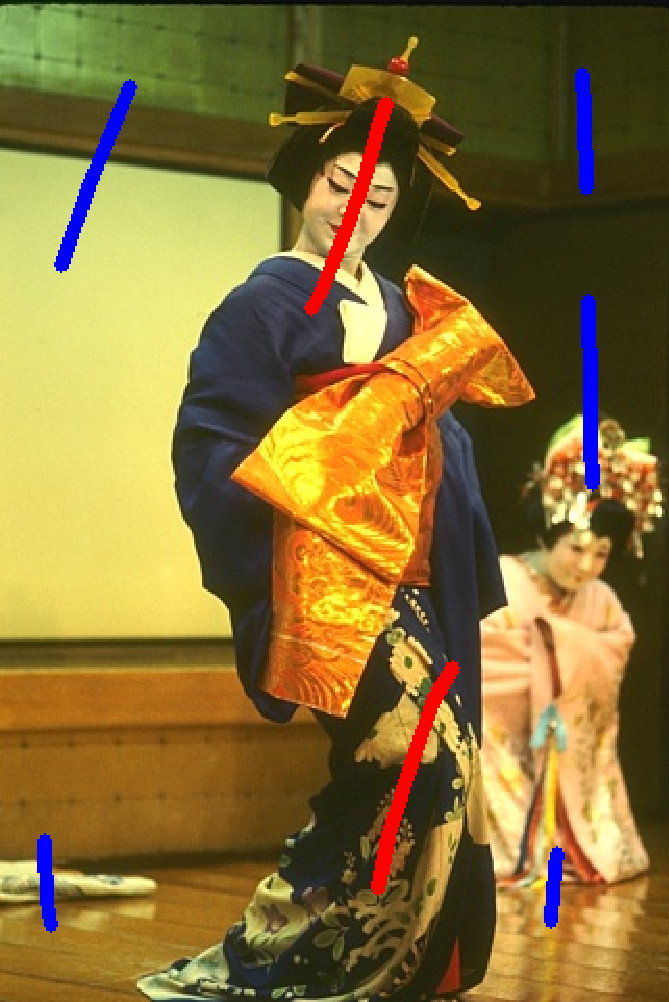
\includegraphics[width=0.23\linewidth]{Figures/5a_1.pdf}}
\subfigure{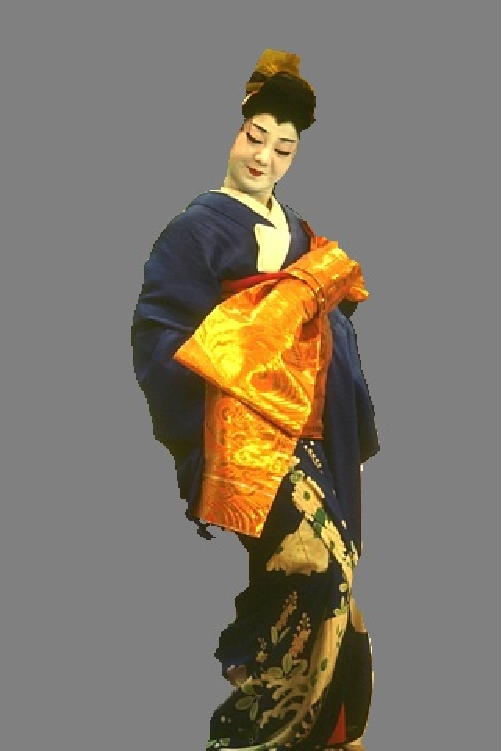
\includegraphics[width=0.23\linewidth]{Figures/5a_2.pdf}}
\subfigure{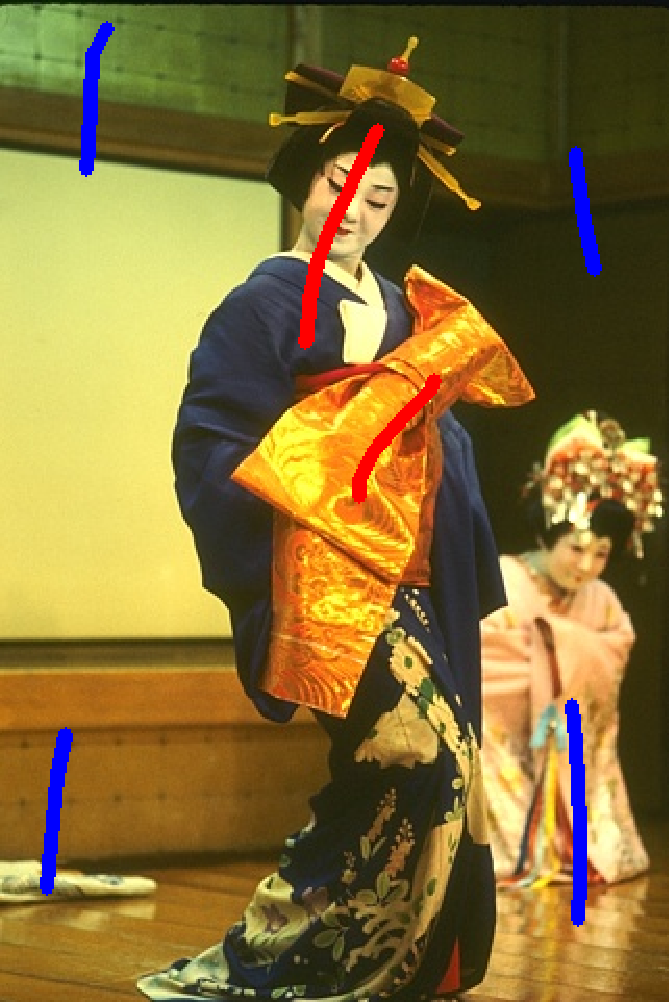
\includegraphics[width=0.23\linewidth]{Figures/5b_1.pdf}}
\subfigure{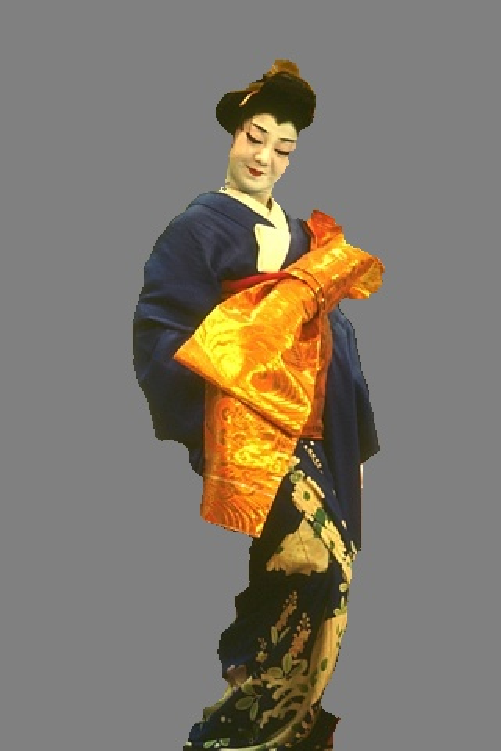
\includegraphics[width=0.23\linewidth]{Figures/5b_2.pdf}}
   \caption{With different inputs (same with Fig~\ref{fig:fig1}), the segmentation results of proposed method are satisfying and similar.}
\label{fig:fig5}
\end{figure}

\begin{table}[!htb]
    \begin{center}
        \begin{tabular}{|c|c|}
        \hline
        Method & error rate (\%)\\
        \hline \hline
        Grabcut\cite{rother2004grabcut} & 5.66 (reported in \cite{nguyen2012robust}) \\
        RW with AT\cite{duchenne2008segmentation} & 3.3 (reported in \cite{duchenne2008segmentation})\\
        Constrained ACM\cite{nguyen2012robust} & 3.77 (reported in \cite{nguyen2012robust}) \\
        Constrained ACM\cite{nguyen2012robust} & 5.06 (with sparse inputs) \\
        Our Method & \textbf{4.30} (with sparse inputs)\\
        Our Method & \textbf{2.78} (with normal inputs)\\
        \hline
        \end{tabular}
    \end{center}
    \vspace{-2em}
    \caption{\small{Error rate comparison using the MSRC dataset}}
    \label{table:tableerrorrate_mstc}
\end{table}
We test and compare the proposed algorithm with other methods on the commonly used MSRC ground truth data set~\cite{rother2004grabcut}, which contains 50 test images with ground truth provided. Table~\ref{table:tableerrorrate_mstc} reports the error rates (percentage of mislabeled pixels) with existing methods and our proposed method. The error rate is the average result of 50 images in MSRC dataset. We tested the Constrained Active Contour Model (Constrained ACM) with both normal inputs and sparse inputs for comparison. From the table, we can see that the proposed method achieves low error rates with sparse and normal inputs, less than those of Constrained ACM \cite{nguyen2012robust} under the same condition. All the input sparse strokes and the segmentation results are supplied in \cite{sub}. The performances of Grabcut\cite{rother2004grabcut}, RW with AT\cite{duchenne2008segmentation} and Constrained ACM\cite{nguyen2012robust} are under the same conditions as where they are reported.
 %Compared \cite{nguyen2012robust} with our method, we can find that the extension for the model on the local and global aspects gained 9.09\% of the performance improvement.

%In Fig.~\ref{fig:fig4}, the segmentation results of complicated foreground or background cases, such as (a), (b) and (c) and the results of similar foreground and background cases, such as (d) are shown. From the segmentation results, we can find that in the complicated cases, the independent regions of foreground without seeds are possibly regarded as background due to the texture and differences of color. When we add the geodesic energy term, the texture structure around with foreground seeds can benefit the regions which are in the local area of seeds. In the cases of similar foreground and background, the model in \cite{nguyen2012robust} hardly find the real contour of foreground object and  even entirely fail in some particular cases with only segmenting the stroke region, like Fig.~\ref{fig:fig4}(d).
%We also evaluate different results in different value of $\lambda_2$ and show the comparison in Fig.~\ref{fig:fig4}. When the $\lambda_2$ is too small, the geodesic energy can not take important effect, but too large value makes the position of seeds too dominant to obtain accurate segmentation. Finally, we set $\lambda_2$ to 1000 in our experiments.
%
The proposed method needs to iteratively refine the seeds and optimize Eq.~\eqref{eq:newmodel} several times, However, the numerical algorithm is very fast and the value of $u$ from the last iteration is a very good initial value, and thus the segmentation can be obtained in real time. The computation time of the examples shown in Fig.~\ref{fig:fig4} are listed in Table\ref{table:time}. All the tests were run on a desktop with an Inter Core i7-3770K CPU and 32GB RAM.
\vspace{-3mm}
\begin{table}[!htb]
    \begin{center}
        \begin{tabular}{|c|c|c|}
        \hline
        Image & Size & time (s)\\
        \hline \hline \hline
        Fig.~\ref{fig:fig4} (1) & $481\times321$ &  1.453\\
        Fig.~\ref{fig:fig4} (2) & $481\times321$ &  1.829\\
        Fig.~\ref{fig:fig4} (3) & $321\times481$ &  1.622\\
        Fig.~\ref{fig:fig4} (4) & $481\times321$ &  1.560\\
        \hline
        \end{tabular}
    \end{center}
    \vspace{-2em}
    \caption{\small{Computation time of the examples in Fig.~\ref{fig:fig4}.}}
    \label{table:time}
\end{table}
%
\vspace{-8mm}
\section{Conclusions}
\label{sec:Conc}
%
In this paper, we proposed an iterative refinement framework with geodesic distance enhancement active contour model. The iterative seeds refinement strategy gradually update the reliable segment part and use them as guidance to segment the unreliable part. With these two newly added strategies, proposed method can handle images with complex textures with low quality and small quantity of input seeds. Experiments on public image segmentation dataset and natural images indicate that our proposed method can achieve high quality segmentation. For future work, it would be interesting to extend the proposed method to multi-class image segmentation.
%
% References should be produced using the bibtex program from suitable
% BiBTeX files (here: refs). The IEEEbib.bst bibliography
% style file from IEEE produces unsorted bibliography list.
% -------------------------------------------------------------------------
\bibliographystyle{IEEEbib}
\bibliography{refs}
%
\end{document}
